\subsection{Конечные размеры источника и пространственная когерентность}


\textbf{Два точечных источника}.
Рассмотрим интереференцию света от двух источников $A$ и $B$ (рис. \eqref{fig281}). 
\begin{figure}[ht]
    \centering
    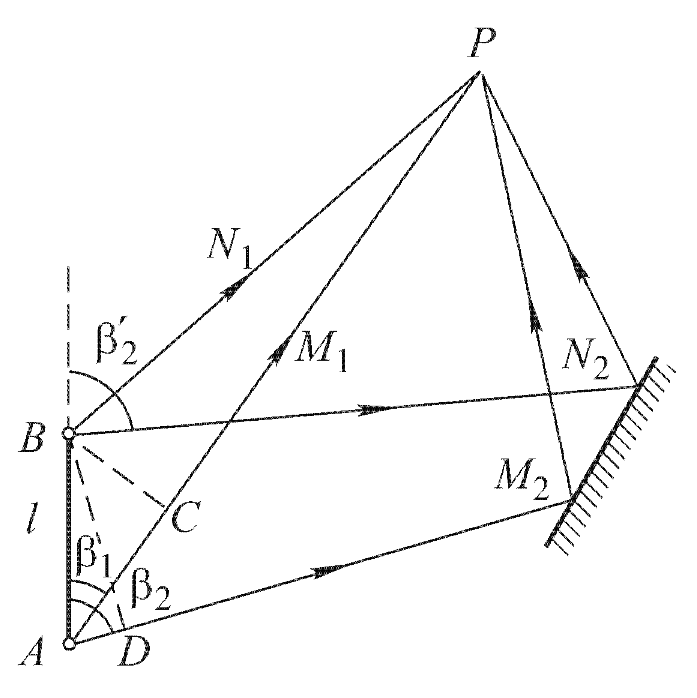
\includegraphics[width=0.3\textwidth]{figures/28_1.png}
    \hspace{5 mm} 
    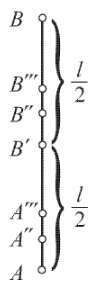
\includegraphics[width=0.09\textwidth]{figures/28_2.png}
    \caption{К пространственной когерентности}
    \label{fig281}
\end{figure}
Считая $l=AB$ достаточно малым, то для разности оптических лучей можно написать $l\cos \beta_1$ и $l \cos \beta_2$. Тогда для разности оптической разности хода лучей от $A$ и $B$ верно, что
\begin{equation*}
    \Delta = 
    \left[(AM_1P)-(AM_2P)\right]-\left[(BN_1 P) - (BN_2P)\right]
   = l |\cos \beta_1 - \cos \beta_2|,
\end{equation*}
которая определяет сдвиг одной интерфереционной картины относительно другой. При $\Delta = \lambda/2$ максимумы одной -- минимумы другой, при $\Delta = \lambda$ резонируют. 

Стоит заметить, что мы условно считаем, что при $\Delta = (m+1/4)\lambda,\, m \in \mathbb{Z}$ -- всё хорошо. А ещё $\beta = \beta'$. 



\textbf{Протяженный источник}.  Считая, что все точки излучают некогерентно, разобьём на пары источников $(A, B'),\,  (A'', B'')$ и т.д. находящиъся на $l/2$ друг от друга. Тогда, при $\Delta/2 = \lambda/2$ от каждой пары будет просто светлый фон, получаем условия
\begin{equation*}
    \Delta \equiv l(\cos \beta_2 - \cos \beta_2) = m\lambda,
\end{equation*}
при выполнении которого на экране один только освещенный фон без полос. При $\Delta = (m+\alpha)\lambda$ источник можно разбить на две части $m \colon  \alpha$, где меньшая часть источника даст интерференционные полосы на светлом фоне от большей части источника. 

Если крайние лучи выходят симметрично к $\bot AB$, т.е. $\beta_2 = \pi-\beta_1$, то $\cos \beta_2 = - \cos \beta_1$, и тогда хорошая интерференция будет при
\begin{equation*}
    (l/2) |cos\beta_1-\cos \beta_2| \leq \lambda/4,
    \hspace{10 mm} 
    l \sin (\Omega/2) \leq \lambda/4,
\end{equation*}
где $\Omega$ -- угол между крайними лучами, угол интерференциии. 


\begin{to_def}
    Два источника, позволяющие наблюдать интереференцию света от них, называют \textit{пространственно когерентными}, иначе -- \textit{пространственно некогерентными}. 
\end{to_def}

В случае жемонохроматичного света, можем говорить про пространственную когерентность при 
\begin{equation*}
    \sigma =\pi \lambda^2 / (4 \varphi^2). 
\end{equation*}